%%%%%%%%%%%%%%%%%%%%%%%%%%%%%%%%%%%%%%%%%%%%%%%%%%%%%%%%%%%%%%%%%%%%%%%%%
%
% Presentation template for Scientific Computing seminar
%
%%%%%%%%%%%%%%%%%%%%%%%%%%%%%%%%%%%%%%%%%%%%%%%%%%%%%%%%%%%%%%%%%%%%%%%%%

\documentclass[hyperref={bookmarks=false},11pt,dvipsnames]{beamer}
\usepackage{tabularx}
\usepackage[linesnumbered,ruled,vlined]{algorithm2e}
\usepackage{hyperref}
\setbeamercolor{url}{fg=red}
\usepackage{mathtools}
\definecolor{buwgreen}{rgb}{0.537,0.729,0.090}
\definecolor{darkred}{rgb}{0.8, 0, 0}

%%%%%%%%%%%%%%%%%%%%%%%%%%%%%%%%%%%%%%%%%%%%%%%%%%%%%%%%%%%%%%%%%%%%%%%%%
% Course metadata
\newcommand{\coursename}{Bachelor-Seminar \glqq{}Top 10 Algorithms in Data Mining\grqq{}}
\newcommand{\coursenamefootline}{Bachelor-Seminar \glqq{}Top 10 Algorithms in Data Mining\grqq{}}

% In seminars, the presenter of a talk is typically different from the lecturer responsible for the course.
% The following commands allow to have this distinction. The lecturer's name is printed in the banner on the 
% titlepage (if activated) and the presenter's name is passed into the \author{} command.
\newcommand{\presentername}{Marius Graf}
\newcommand{\presenternameshort}{M. Graf}
\newcommand{\lecturername}{Dr.~Marcel Schweitzer}

\author[\presenternameshort]{\presentername}
\institute{Bergische Universität Wuppertal}
\def\englishlanguage{0}             % set to 1 to switch from German to English

%%%%%%%%%%%%%%%%%%%%%%%%%%%%%%%%%%%%%%%%%%%%%%%%%%%%%%%%%%%%%%%%%%%%%%%%%
% Switches for title page design
\def\printbanner{1}                 % set to 1 to print title page banner
\def\printauthor{1}                 % set to 1 if author name should also be printed outside of title banner
\def\printdate{1}                   % set to 1 in order to print date
\def\printinstitute{0} 		          % set to 1 in order to print institute
\def\printcoursename{1}		          % set to 1 to print course name above title and in footline

%%%%%%%%%%%%%%%%%%%%%%%%%%%%%%%%%%%%%%%%%%%%%%%%%%%%%%%%%%%%%%%%%%%%%%%%%
% Other layout switches
\def\coveredtransparent{1}          % set to 1 to make covered items completely invisible
\def\printnavigationsymbols{0}      % set to 1 to activate navigation symbols
\def\printtocatbeginofsection{1}    % print outline slide (with highlighted current section) at beginning of each section
\def\printtocatbeginofsubsection{0} % print outline slide (with highlighted current subsection) at beginning of each subsection
\def\printlion{1}                   % set to 0 to suppress small "Uni-Loewe" icon in top right corner
\def\printpagenumbers{1}            % set to 0 to suppress page numbers in foot line
\def\longtitle{0}                   % Sometimes, very long titles can break the title page layout. In that case, setting this to 1 might improve things

%%%%%%%%%%%%%%%%%%%%%%%%%%%%%%%%%%%%%%%%%%%%%%%%%%%%%%%%%%%%%%%%%%%%%%%%%
\usetheme{HPC}

% Set language options
\if\englishlanguage0
	\PassOptionsToPackage{german,germankw,onelanguage}{algorithm2e}
	\PassOptionsToPackage{ngerman}{babel}
\else
	\PassOptionsToPackage{english}{babel}
\fi

%%%%%%%%%%%%%%%%%%%%%%%%%%%%%%%%%%%%%%%%%%%%%%%%%%%%%%%%%%%%%%%%%%%%%%%%%
% Include useful packages 
\usepackage[utf8]{inputenc}
\usepackage{amsmath}
\usepackage{framed}
\usepackage[ruled,vlined]{algorithm2e}
\usepackage{amssymb}
\usepackage{array}
\usepackage{caption}
\usepackage{bbding}
\usepackage{bm}
\usepackage{hyperref}
\usepackage{tikz}
\usepackage{times}
\usepackage{ifthen}
\usepackage{pgfplots}
\usepackage{alltt}
\usepackage{transparent}
\usepackage{colortbl}
\usepackage{textcomp}
\usepackage{multirow}
\usepackage{babel}


% increase itemize spacing
\let\realitemize\itemize
\let\endrealitemize\enditemize
\renewenvironment{itemize}{%
	\realitemize\setlength{\parskip}{0pt}\setlength{\itemsep}{.24cm}}
{%
	\endrealitemize%
}

% Switch between transparency and invisibility for covered things
\if\coveredtransparent1
	\setbeamercovered{transparent}
\fi

%%%%%%%%%%%%%%%%%%%%%%%%%%%%%%%%%%%%%%%%%%%%%%%%%%%%%%%%%%%%%%%%%%%%%%%%%
% TikZ initializations, in particular for overlays and externalization

\pgfplotsset{compat=1.12}

\tikzstyle{every picture}+=[remember picture]
\tikzstyle{na} = [baseline=-.5ex, xshift = -0.15cm]
\tikzstyle{na2} = [baseline=-.5ex, xshift = -0.35cm]

\tikzset{
	ncbar angle/.initial=90,
	ncbar/.style={
			to path=(\tikztostart)
			-- ($(\tikztostart)!#1!\pgfkeysvalueof{/tikz/ncbar angle}:(\tikztotarget)$)
			-- ($(\tikztotarget)!($(\tikztostart)!#1!\pgfkeysvalueof{/tikz/ncbar angle}:(\tikztotarget)$)!\pgfkeysvalueof{/tikz/ncbar angle}:(\tikztostart)$)
			-- (\tikztotarget)
		},
	ncbar/.default=0.5cm,
}

\tikzset{square left brace/.style={ncbar=0.5cm}}
\tikzset{square right brace/.style={ncbar=-0.5cm}}

\tikzset{round left paren/.style={ncbar=0.5cm,out=120,in=-120}}
\tikzset{round right paren/.style={ncbar=0.5cm,out=60,in=-60}}
\usetikzlibrary{positioning,matrix,arrows,arrows.meta,backgrounds,shapes}
\usetikzlibrary{backgrounds,mindmap,decorations.pathreplacing,external,calc}
\tikzexternalize[prefix=tikzfigures/] % path for saving precompiled tikz pictures

% Command for easily connecting tikz anchors on slide by arrow
\newcommand{\connectbyarrow}[3]{%
	\begin{tikzpicture}[overlay]
		\path[->,UniGruen,very thick,shorten >= .25cm, shorten <= .25cm] (#1) edge [#3] (#2);
	\end{tikzpicture}
}

%%%%%%%%%%%%%%%%%%%%%%%%%%%%%%%%%%%%%%%%%%%%%%%%%%%%%%%%%%%%%%%%%%%%%%%%%
% Some layout stuff

% set custom text margins
\setbeamersize{text margin left=1em,text margin right=1em}

% Turn off navigation symbols if desired
\if\printnavigationsymbols0
	\beamertemplatenavigationsymbolsempty
\fi

% footline design
\setbeamertemplate{footline}{
	\begin{beamercolorbox}[sep=2pt]{footline}
		\hspace{1em}\insertshortauthor\\ \textit{\insertshorttitle{} \ifthenelse{\printcoursename=1}{(\coursenamefootline)}{}} \hfill
		\ifthenelse{\printpagenumbers=1}{\insertframenumber/\inserttotalframenumber}{} \hspace{1pt}
	\end{beamercolorbox}
}

% custom commands for removing some slides from miniframes (needed for table of contents
% at beginning of section/subsection, see below)
\makeatletter
\let\beamer@writeslidentry@miniframeson=\beamer@writeslidentry
\def\beamer@writeslidentry@miniframesoff{%
	\expandafter\beamer@ifempty\expandafter{\beamer@framestartpage}{}%
	{%
		\clearpage\beamer@notesactions%
	}
}
\newcommand*{\miniframeson}{\let\beamer@writeslidentry=\beamer@writeslidentry@miniframeson}
\newcommand*{\miniframesoff}{\let\beamer@writeslidentry=\beamer@writeslidentry@miniframesoff}
\beamer@compresstrue
\makeatother

% Print table of contents at beginning of each section, with the current section highlighted in green and everything else shaded
\if\printtocatbeginofsection1
	\AtBeginSection[]
	{
		% Remove frame number from footline on outline slides
		\let\rememberpagenumberswitch\printpagenumbers
		\def\printpagenumbers{0}
		\miniframesoff
		\begin{frame}[t,noframenumbering]{\ifthenelse{\englishlanguage=1}{Outline}{Inhalt}}
			\setbeamercolor{section in toc}{fg=UniGruen,bg=}
			\setbeamercolor{section in toc shaded}{fg=Gray,bg=}
			\setbeamercolor{subsection in toc shaded}{fg=Gray,bg=}
			\setbeamercolor{subsection in toc}{fg=Gray,bg=}
			\tableofcontents[currentsection]
		\end{frame}
		\miniframeson
		\let\printpagenumbers\rememberpagenumberswitch
	}
\fi

% Print table of contents at beginning of each subsection, with the current section and subsection highlighted in green and everything else shaded
\if\printtocatbeginofsubsection1
	\AtBeginSubsection[]
	{
		% Remove frame number from footline on outline slides
		\let\rememberpagenumberswitch\printpagenumbers
		\def\printpagenumbers{0}
		\miniframesoff
		\begin{frame}[t,noframenumbering]{\ifthenelse{\englishlanguage=1}{Outline}{Inhalt}}
			\setbeamercolor{section in toc}{fg=UniGruen,bg=}
			\setbeamercolor{section in toc shaded}{fg=Gray,bg=}
			\setbeamercolor{subsection in toc shaded}{fg=Gray,bg=}
			\setbeamercolor{subsection in toc}{fg=UniGruen,bg=}
			\tableofcontents[currentsection,currentsubsection]
		\end{frame}
		\miniframeson
		\let\printpagenumbers\rememberpagenumberswitch
	}
\fi

% Include small "Uni-Loewe" icon in top right corner of each slide
\if\printlion1
	\addtobeamertemplate{frametitle}{}{%
		\tikzexternaldisable%
		\begin{tikzpicture}[remember picture,overlay]%
			\node[anchor=north east,yshift=1.5pt, xshift = 0.2pt] at (current page.north east) {
\includegraphics[height=.6cm]{figures/loewe-weiss.pdf}};%
		\end{tikzpicture}%
		\tikzexternalenable%

		\vspace{-.5cm}
	}
\fi

%%%%%%%%%%%%%%%%%%%%%%%%%%%%%%%%%%%%%%%%%%%%%%%%%%%%%%%%%%%%%%%%%%%%%%%%%
% Title page

% Do not count title page in page numbering
\let\otp\titlepage
\renewcommand{\titlepage}{\otp\addtocounter{framenumber}{-1}}

% Custom title page layout
\defbeamertemplate*{title page}{customized}
{
	\thispagestyle{empty}

	%\vspace{-.5cm}
	\if\printbanner1
		\hpcbanner
	\fi

	\vspace*{.25cm}
	\begin{center}
		\if\printcoursename1
			\Large\textbf{\coursename}\par
		\fi
		\bigskip
		\hfill
		\begin{beamercolorbox}[rounded=true, center, wd=.8\paperwidth]{mycolor}
			\Large\inserttitle
		\end{beamercolorbox}
		\hfill\hfill

		\bigskip
		\bigskip

		\if\printauthor1
			\normalsize\textbf{\insertauthor}\par
		\fi

		\vspace{.15cm}
		\bigskip
		\if\printinstitute1
			\small\insertinstitute\par
		\fi
		\bigskip
		\if\printdate1
			\normalsize\insertdate\par
		\fi
		\ifx\longtitle\undefined
		\else
			\if\longtitle1
				\vspace{-1cm}
			\else

			\fi
		\fi
	\end{center}
}

% Generate HPC banner for title page, similar to our exercise sheet headers etc.
\newcommand{\hpcbanner}{
	\makebox[\textwidth][c]{
		\begin{tikzpicture}
			[textnode/.style={white,font={\bf \sffamily \small},inner sep=0pt}]
			\fill [UniGruen] (0,0) rectangle (\paperwidth,2cm);
			\node [inner sep=0pt] (loewe) at (1,1) {
\includegraphics[width=1.75cm]{figures/loewe-weiss.pdf}};
			\node [textnode,anchor=west] (T) at (2.25,1) {\ifthenelse{\englishlanguage=1}{Scientific Computing \& High Performance Computing}{Wissenschaftliches Rechnen und Hochleistungsrechnen}};
			\node [textnode,above=0.6cm of T.west,anchor=west] {Bergische Universität Wuppertal};
			\node [textnode,below=0.6cm of T.west,anchor=west] {\lecturername};
		\end{tikzpicture}
	}
}

%%%%%%%%%%%%%%%%%%%%%%%%%%%%%%%%%%%%%%%%%%%%%%%%%%%%%%%%%%%%%%%%%%%%%%%%%
% Auxiliary stuff

% Remove algorithm numbering
\renewcommand{\thealgocf}{}

% Command for including small book icon that can be used for referencing literature, lecture notes or similar
\newcommand{\smallbook}{
\includegraphics[width = .028\textwidth]{figures/bookicon.pdf}}

% Command that generates a framed box containing a book icon and text
\newcommand{\inbook}[1]{{\setlength{\topsep}{0pt}
			\begin{framed}
				\begin{minipage}{.08\textwidth}
					
\includegraphics[width = .99\textwidth]{figures/bookicon.pdf}
				\end{minipage}
				\begin{minipage}{.9\textwidth}
					#1
				\end{minipage}
			\end{framed}}}

% Slight change of bibliography layout to look better on slides
\let\OLDthebibliography\thebibliography
\renewcommand\thebibliography[1]{
	\OLDthebibliography{#1}
	\setlength{\parskip}{0pt}
	\setlength{\itemsep}{0pt plus 0.3ex}
}

%%%%%%%%%%%%%%%%%%%%%%%%%%%%%%%%%%%%%%%%%%%%%%%%%%%%%%%%%%%%%%%%%%%%%%%%%
% Some commands that I frequently need
\newcolumntype{C}[1]{>{\centering\arraybackslash}p{#1}}
% Define your logos here to be used on the title page
\newcommand{\BUWLogo}{
\includegraphics[height=32pt]{figures/loewe-weiss.pdf}}
\newcommand{\upk}{^{(k)}}
\newcommand{\upm}{^{(m)}}
\newcommand{\upinv}{^{-1}}
\newcommand{\R}{\mathbb{R}}
\newcommand{\N}{\mathbb{N}}
\newcommand{\C}{\mathbb{C}}
\newcommand{\K}{\mathcal{K}}
\newcommand{\bigO}{\mathcal{O}}
\newcommand{\Rn}{\mathbb{R}^n}
\newcommand{\Rk}{\mathbb{R}^k}
\newcommand{\Cn}{\mathbb{C}^n}
\newcommand{\Rnn}{\mathbb{R}^{n \times n}}
\newcommand{\Cnn}{\mathbb{C}^{n \times n}}
\newcommand{\slitplane}{\mathbb{C} \setminus \mathbb{R}_0^-}
\newcommand{\va}{{\mathbf a}}
\newcommand{\vb}{{\mathbf b}}
\newcommand{\vc}{{\mathbf c}}
\newcommand{\vd}{{\mathbf d}}
\newcommand{\vdhat}{{\mathbf {\hat d}}}
\newcommand{\ve}{{\mathbf e}}
\newcommand{\vehat}{{\mathbf {\hat e}}}
\newcommand{\vf}{{\mathbf f}}
\newcommand{\vftilde}{{\mathbf {\widetilde f}}}
\newcommand{\vg}{{\mathbf g}}
\newcommand{\vh}{{\mathbf h}}
\newcommand{\vhhat}{{\mathbf {\hat h}}}
\newcommand{\vk}{{\mathbf k}}
\newcommand{\vp}{{\mathbf p}}
\newcommand{\vq}{{\mathbf q}}
\newcommand{\vr}{{\mathbf r}}
\newcommand{\vs}{{\mathbf s}}
\newcommand{\vt}{{\mathbf t}}
\newcommand{\vu}{{\mathbf u}}
\newcommand{\vv}{{\mathbf v}}
\newcommand{\vw}{{\mathbf w}}
\newcommand{\vx}{{\mathbf x}}
\newcommand{\vy}{{\mathbf y}}
\newcommand{\vz}{{\mathbf z}}
\newcommand{\vnull}{\boldsymbol{0}}
\newcommand{\vone}{\boldsymbol{1}}
\newcommand{\spK}{{\cal K}}
\newcommand{\spEK}{{\cal E}}
\newcommand{\spL}{{\cal L}}
\newcommand{\spP}{{\cal P}}
\newcommand{\tol}{\texttt{tol}{}}
\newcommand{\specialcell}[2][l]{\begin{tabular}[#1]{@{}c@{}}#2\end{tabular}}
\renewcommand{\d}{\,\mathrm{d}}
\newcommand{\dmu}{\d\mu(t)}
\newcommand{\dalpha}{\d\alpha(z)}
\DeclareMathOperator{\Pe}{Pe}
\DeclareMathOperator{\spec}{spec}
\DeclareMathOperator{\diag}{diag}
\DeclareMathOperator{\range}{range}
\DeclareMathOperator{\Span}{span}
\DeclareMathOperator{\trace}{trace}
\DeclareMathOperator{\tr}{tr}
\DeclareMathOperator{\sign}{sign}
\DeclareMathOperator*{\argmin}{arg\,min}
\DeclareMathOperator*{\argmax}{arg\,max}
\newcommand{\lmin}{{\lambda_{\min}}}
\newcommand{\lmax}{{\lambda_{\max}}}
\newcommand{\AHA}{A^H\!A}
\newcommand{\tve}{\widetilde{{\mathbf e}}}
\newcommand{\tvf}{\widetilde{{\mathbf f}}}
\newcommand{\tvx}{\widetilde{{\mathbf x}}}
\newcommand{\tvr}{\widetilde{{\mathbf r}}}
\newcommand{\rhoinvA}{\rho}
\newcommand{\deltaA}{\delta}
\newcommand{\deltainvA}{\delta'}
\newcommand{\Lmax}{\Lambda_{\max}}
\newcommand{\nmin}{\nu_{\min}}
\newcommand{\nmax}{\nu_{\max}}
\newcommand{\calO}{\mathcal{O}}
\newcommand{\comment}[1]{{\small\color{gray!50}// #1}}
\DeclareMathAlphabet{\mathbf}{OT1}{cmr}{bx}{n}
\def\Hat{\mkern-3mu\text{\textasciicircum}}
 
% \DeclareMathOperator*{\sign}{sign}

\title{AdaBoost}
\date{06.12.2023}


\begin{document}

%%%%%%%%%%%%%%%%%%%%%%%%%%%%%%%%%%%%%%%%%%%%%%%%%%%%%%%%%%%%%%%%
% title slide
\maketitle
%%%%%%%%%%%%%%%%%%%%%%%%%%%%%%%%%%%%%%%%%%%%%%%%%%%%%%%%%%%%%%%%


%%%%%%%%%%%%%%%%%%%%%%%%%%%%%%%%%%%%%%%%%%%%%%%%%%%%%%%%%%%%%%%%
% outline slide (without frame number in foot line)
\let\rememberpagenumberswitch\printpagenumbers
\def\printpagenumbers{0}

\begin{frame}[t,noframenumbering]{\ifthenelse{\englishlanguage=1}{Outline}{Inhalt}}
	\tableofcontents
\end{frame}
\let\printpagenumbers\rememberpagenumberswitch
%%%%%%%%%%%%%%%%%%%%%%%%%%%%%%%%%%%%%%%%%%%%%%%%%%%%%%%%%%%%%%%%


%%%%%%%%%%%%%%%%%%%%%%%%%%%%%%%%%%%%%%%%%%%%%%%%%%%%%%%%%%%%%%%%%%%%%%%%%
%
% Content starts here
%
%%%%%%%%%%%%%%%%%%%%%%%%%%%%%%%%%%%%%%%%%%%%%%%%%%%%%%%%%%%%%%%%%%%%%%%%%

\section{Einleitung}

\begin{frame}[t]{Was ist Data Mining?}
	
\includegraphics[width=0.5\textwidth]{figures/datamining.png}
	\begin{itemize}
		\item <1-> \textbf{Analysiert} große Datenmengen, um Muster und Zusammenhänge zu erkennen.
		\item <2-> Nutzt dabei Methoden aus der \textbf{Statistik}, dem  \textbf{Machine Learning} und Datenbanktechnologien.
		\item <3-> Spielt zentrale Rolle in der Forschung und Industrie,
		      um Erkenntnisse zu gewinnen und
		      Entscheidungen zu unterstützen.
	\end{itemize}
\end{frame}
\begin{frame}[t]{Was sind Ensemble-Methoden?}
	\begin{itemize}
		\item <1-> \textbf{Ensemble-Verfahren:} \textbf{Kombinieren} mehrere Modelle für präzisere Vorhersagen
		\item <2-> \textbf{Fehlerminimierung:} Reduzieren von \textbf{systematischen Fehlern} in Modellprognosen
		\item <3-> \textbf{Arten von Ensemble-Methoden:}\\[5pt]
		      \begin{itemize}
			      \item Bagging
			      \item Stacking
			      \item Boosting
		      \end{itemize}
		\item <4-> \textbf{AdaBoost gehört zu den Boosting-Verfahren}
	\end{itemize}
\end{frame}

\section{Grundlagen des Boosting}
\begin{frame}[t]{Die Grundidee}
	\begin{itemize}
		\item <1-> Boosting kombiniert \textbf{schwache Lerner} zu einem \textbf{starken Gesamtmodell}
		\item <2-> \textbf{Schwacher Lerner:} Modell, das nur \textbf{geringfügig besser} ist als \textbf{zufälliges Raten}
		\item <3-> \textbf{Passe Gewichtung} der Trainingsdaten iterativ \textbf{an}, damit neue Modelle die \textbf{Fehler der Vorgänger korrigieren}
		\item <4-> $\leadsto$ verringerter \textbf{Bias, bessere Vorhersagegenauigkeit} für schwer klassifizierbare Beispiele
	\end{itemize}
\end{frame}

\begin{frame}[t]{Veranschaulichung}
	\centering
	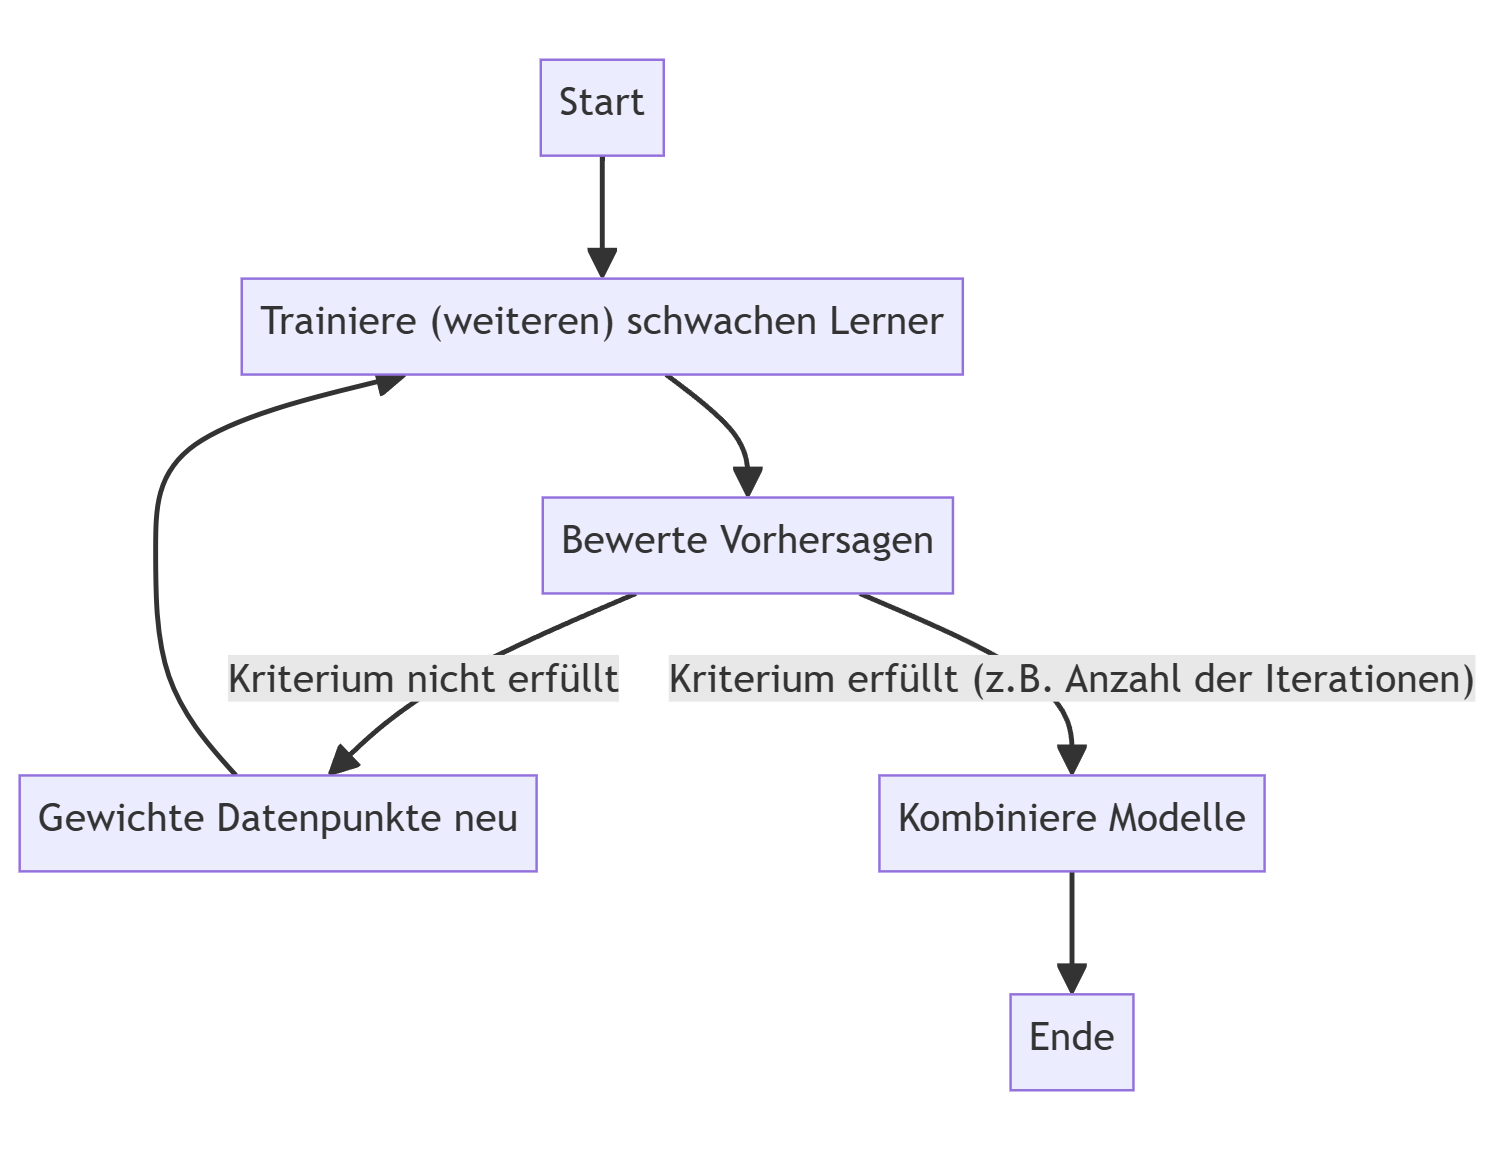
\includegraphics[width=0.8\textwidth]{../Ausarbeitung/figures/Boosting_Graph.png}
\end{frame}
\begin{frame}[t]{Beispiel}{Vorhersage von Hauspreisen}
	\begin{itemize}
		\item <1-> Wir möchten ein \textbf{Modell} entwickeln, das den \textbf{Preis von
			      Häusern} basierend auf \textbf{verschiedenen Merkmalen} wie Größe, Lage, Anzahl der
		      Zimmer und Baujahr \textbf{vorhersagt}.
	\end{itemize}
	\begin{table}
		\centering
		\resizebox{\textwidth}{!}{%
			\begin{tabularx}{\textwidth}{|X|X|X|X|}
    \hline
    \textbf{Haus} & \textbf{Größe $[m^2]$} & \textbf{Lage} & \textbf{Preis} \\
    \hline
    Haus 1        & 100                    & Zentrum       & 500.000€       \\
    \hline
    Haus 2        & 150                    & Vorort        & 300.000€       \\
    \hline
    Haus 3        & 80                     & Zentrum       & 400.000€       \\
    \hline
    Haus 4        & 120                    & Ländlich      & 200.000€       \\
    \hline
\end{tabularx}
		}
	\end{table}


\end{frame}
\subsection*{Beispiel}
\begin{frame}[t]{Beispiel}{Vorhersage von Hauspreisen}
	\begin{itemize}
		\item <1-> \textbf{Einfaches Modell} (schwacher Lerner): Preisvorhersage nur anhand von \textbf{Größe}
		\item <2-> Tatsächlich spielen auch \textbf{andere Faktoren} (z.B. Lage) eine Rolle
		\item <3-> $\leadsto$ \textbf{Bias} des schwachen Lerners:\\[5pt]
		      \begin{itemize}
			      \item Preis von Häusern in guter Lage wird \textbf{unterschätzt}
			      \item Preis von Häusern in schlechter Lage wird \textbf{überschätzt}
		      \end{itemize}
	\end{itemize}
\end{frame}

\begin{frame}[t]{Beispiel}{Vorhersage von Hauspreisen}
	\begin{itemize}
		\item \textbf{Boosting:} Passe iterativ Gewicht der Datenpunkte so an, dass nächstes Modell verstärkt die schlecht vorhergesagten Fälle beachtet
		\item [] \emph{P = Vorhersage, W = Gewichtung}
	\end{itemize}
	\begin{table}
		\centering
		\resizebox{0.95\textwidth}{!}{%
			\begin{tabularx}{\textwidth}{|X|X|X|X|X|X|}
    \hline
    \textbf{Haus} & \textbf{Größe $[m^2]$} & \textbf{Lage} & \textbf{Preis} & \textbf{Vorhersage (It. 1)} & \textbf{Vorhersage (It. 2)} \\
    \hline
    Haus 1        & 100                    & Zentrum       & 500.000€       & 450.000€                    & 490.000€                    \\
    \hline
    Haus 2        & 150                    & Vorort        & 300.000€       & 350.000€                    & 310.000€                    \\
    \hline
    Haus 3        & 80                     & Zentrum       & 400.000€       & 380.000€                    & 405.000€                    \\
    \hline
    Haus 4        & 120                    & Ländlich      & 200.000€       & 250.000€                    & 210.000€                    \\
    \hline
\end{tabularx}
		}
		\resizebox{0.95\textwidth}{!}{%
			\begin{tabularx}{\textwidth}{|X|X|X|X|X|X|}
    \hline
    \textbf{Haus} & \textbf{P(1)} & \textbf{W(1)} & \textbf{P(2)} & \textbf{W(2)} & \textbf{P(3)} \\
    \hline
    Haus 1        & 450.000€      & 0.1307        & 445.000€      & 0.1192        & 443.000€      \\
    \hline
    Haus 2        & 350.000€      & 0.5299        & 495.000€      & 0.4833        & 501.000€      \\
    \hline
    Haus 3        & 380.000€      & 0.1444        & 430.000€      & 0.1691        & 410.000€      \\
    \hline
    Haus 4        & 250.000€      & 0.1950        & 230.000€      & 0.2283        & 205.000€      \\
    \hline
\end{tabularx}
		}
	\end{table}
\end{frame}

\section{Der AdaBoost Algorithmus}
\begin{frame}[t]{Einführung}
	\begin{itemize}
		\item <1-> \glqq Adaptive Boosting\grqq
		\item <2-> entwickelt in den 1990ern von Freund und Schapire, einflussreiches Verfahren für \textbf{binäre Klassifikation}
		\item <3-> Boosting-Methode, \textbf{Gewichtung} falsch klassifizierter Datenpunkte \textbf{exponentiell} erhöht
		\item <4-> spezielle \textbf{adaptive} Fehlerkorrektur
	\end{itemize}
\end{frame}

\begin{frame}{Vereinfachte Sicht auf den Algorithmus}
	\begin{algorithm}[H]
		\DontPrintSemicolon
		\LinesNotNumbered
		\SetKwInput{KwData}{Daten}
		\SetKwInput{KwResult}{Ergebnis}
		\BlankLine
		\KwIn{Datensatz, Lernalgorithmus}
		Initialisiere Gewichte des Datensatzes\;
		\For{\(t = 1\) \KwTo \(T\)}{
			Trainiere schwache Lerner mit gewichtetem Datensatz\;
			Bestimme Fehler der Lerner\;
			Wähle schwachen Lerner mit geringstem Fehler\;
			Berechne Lernkoeffizienten\;
			Gewichte Datenpunkte neu\;
		}
		\KwOut{\text{Starker Lerner (Ensemble)}}
	\end{algorithm}
\end{frame}

\begin{frame}[t]{Notation}
	\begin{itemize}
		\item <1-> $\mathcal{X}:$ Menge der \textbf{Features}
		\item <2-> $\mathcal{Y}:$ Menge der \textbf{Labels} $(\mathcal{Y}=\{-1,+1\}$ bei binärer Klassifikation)
		\item <3-> $D:$ \textbf{Trainingdatensatz} der Form $D=\{(\boldsymbol{x}_i,y_i)\},~i=1,...,m$
		\item <4-> Modell wird auf $D$ durch \textbf{Lernalgorithmus} $\mathcal{L}$ (meistens \emph{Decision Stump}) trainiert und gibt
		\item <5-> eine \textbf{Hypothese} $h:X\rightarrow\mathcal{Y},~h(\boldsymbol{x})=y$ zurück
		\item <6-> Anzahl der \textbf{Trainingsiterationen} $T$
		\item <7-> bei jeder Iteration wird $D$ um \textbf{Gewichte} $$w^{(t)}_i$$ mit $i=1,\dots,m$ und $t=1,\dots,T$ erweitert
	\end{itemize}
\end{frame}

\begin{frame}[t]{Initialisierung der Gewichte}
	\begin{itemize}
		\item <1-> Zu beginn sind die Gewichte gleich verteilt $$
    \mathcal{D}_1(i) = \frac{1}{m}
$$
		\item <2-> Die Summe der Gewichte ist stets 1 $$
    \sum_{i=1}^m w_i^{(t)}= 1~~\forall t=1,\dots,T
$$
	\end{itemize}
\end{frame}

\begin{frame}[t]{Training der schwachen Lerner}
	\begin{itemize}
		\item <1-> \textbf{Trainiere} pro Iteration $n$ \textbf{schwache Lerner} (für jedes Feature zwei, je mit umgekehrter Polarität)
		      $$
			      h = \mathcal{L}(D, w^{(t)})
		      $$
		      mit $w^{(t)}$ als Gewichte der $t$-ten Iteration
		\item <2-> Ziel: gewichteten \textbf{Fehler minimieren}
		      $$
			      \varepsilon_j = \sum_{i=1}^m w_i^{(t)}\cdot I\left(y_i \neq h_j\left(\boldsymbol{x}_i\right)\right),~j=1,\dots,n
		      $$
		      Wähle Lerner $h_j\in h$ mit \textbf{geringstem Fehler} $\varepsilon_j$ (meiste korrekt klassifizierte Datenpunkte)
		\item <3-> Dabei bezeichntet $I$ die \textbf{Indikatorfunktion}
		      $$
			      I(A)=\left\{\begin{array}{l l}
				      1, & \text{wenn } A \\
				      0, & \text{sonst.}
			      \end{array}\right.
		      $$
	\end{itemize}
\end{frame}

\begin{frame}[t]{Berechnung des Lernkoeffizienten}
	\begin{itemize}
		\item <1-> Exponentieller Verlust \begin{align*}
			      L(h_t) = \sum_{i=1}^{m} w_i^{(t)}e^{-y_ih_t(x_i)}
		      \end{align*}
		\item <2-> Herleitung: führe Lernkoeffizienten $\alpha_t$ ein \begin{align*}
			      L(h_t)=\sum_{i=1}^{m}w_ie^{-\alpha_ty_ih_t(x_i)}
		      \end{align*}
	\end{itemize}
\end{frame}

\begin{frame}[t]{Berechnung des Lernkoeffizienten}
	\begin{itemize}
		\item <1-> [] \begin{align*}
			      y_i = h_t(x_i)    & \implies y_ih_t(x_i)  = 1                                     \\
			                        & \leadsto \text{ Beitrag zum Verlust: } w_i^{(t)}e^{-\alpha_t} \\
			      y_i \neq h_t(x_i) & \implies y_ih_t(x_i)  = -1                                    \\
			                        & \leadsto \text{ Beitrag zum Verlust: } w_i^{(t)}e^{\alpha_t}
		      \end{align*}
		\item <3-> Minimieren von $L(h_t)$:\begin{align*}
			      L(h_t) = \sum_{y_i=h_t(x_i)}w_i^{(t)}e^{-\alpha_t} + \sum_{y_i\neq h_t(x_i)} w_i^{(t)}e^{\alpha_t} \\
		      \end{align*}
		\item<4->[] \begin{align*}
			      \frac{dL(h_t)}{d\alpha_t} = -e^{-\alpha_t}\sum_{y_i=h_t(x_i)}w_i^{(t)} + e^{\alpha_t}\sum_{y_i\neq h_t(x_i)}w_i^{(t)} = 0
		      \end{align*}
	\end{itemize}
\end{frame}

\begin{frame}[t]{Berechnung des Lernkoeffizienten}
	\begin{itemize}
		\item <1-> [] \begin{align*}
			       & \Leftrightarrow e^{2\alpha_t} = \frac{\sum_{y_i=h_t(x_i)}w_i}{\sum_{y_i\neq h_t(x_i)}w_i}                       \\
			       & \Leftrightarrow \alpha_t = \frac{1}{2}\ln\left(\frac{\sum_{y_i=h_t(x_i)}w_i}{\sum_{y_i\neq h_t(x_i)}w_i}\right)
		      \end{align*}
		\item<2-> Da $\sum_{y_i=h_t(x_i)}w_i=1-\varepsilon_t$ und $\sum_{y_i\neq h_t(x_i)}w_i=\varepsilon_t$\begin{align*}
			      \implies \alpha_t =\frac{1}{2}\ln\left(\frac{1-\varepsilon_t}{\varepsilon_t}\right)
		      \end{align*}
	\end{itemize}
\end{frame}

\begin{frame}[t]{Berechnung des Lernkoeffizienten}
	\begin{align*}
		\alpha_t =\frac{1}{2}\ln\left(\frac{1-\varepsilon_t}{\varepsilon_t}\right)
	\end{align*}
	\centering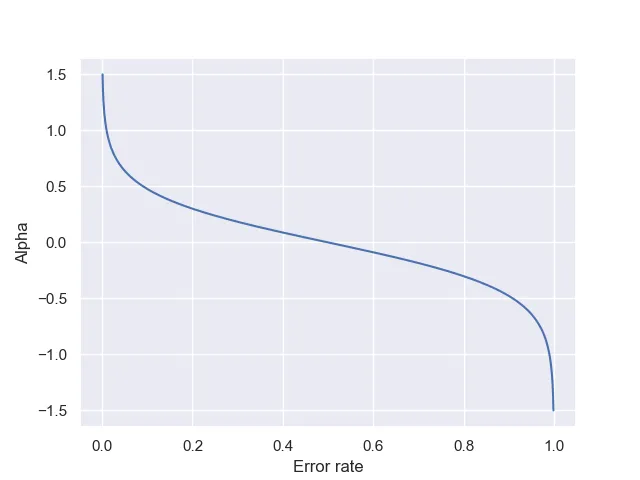
\includegraphics[width=0.6\textwidth]{../Ausarbeitung/figures/alpha_graph.png}
\end{frame}

\begin{frame}[t]{Aktualisierung der Gewichte}
	\begin{itemize}
		\item <1-> Neue Gewichte der Daten für den nächsten Durchlauf berechnen
		      \begin{align*}
			      \begin{array}{l l l}
				      w^{(t+1)}_i & = w^{(t)}_i \cdot e^{-\alpha_t} & \text{für korrekt klassifizierte Datenpunke} \\
				      w^{(t+1)}_i & = w^{(t)}_i \cdot e^{\alpha_t}  & \text{für falsch klassifizierte Datenpunke}
			      \end{array}
		      \end{align*}
		\item <2-> Die neuen Gewichte müssen anschließend normalisiert werden, damit ihre Summe wieder 1 ist:
		      \begin{align*}
			      Z_t         & =\sum_{j=1}^m w^{(t+1)}_i\qquad(\text{Normalisierungsfaktor}) \\
			      w^{(t+1)}_i & = \frac{w^{(t+1)}_i}{Z_t}
		      \end{align*}
	\end{itemize}
\end{frame}

\begin{frame}[t]{Das Ergebnis des Algorithmus}
	Der Algorithmus gibt ein Gesamtmodell zurück, welches die Klassifizierung des Datenpunktes durch die gewichtete
	Summe aller schwachen Lerner darstellt:
	\begin{align*}
		H    & :      X \rightarrow \{-1, +1\}                 \\
		H(x) & =  \sign\left(\sum_{t=1}^T\alpha_th_t(x)\right)
	\end{align*}
\end{frame}

\begin{frame}[allowframebreaks]{Der vollständige Algorithmus}
	\begin{scriptsize}
		\begin{algorithm}[H]
    \DontPrintSemicolon
    \LinesNotNumbered
    \KwData{Trainingsdatensatz \(D\), Anzahl der Iterationen \(T\).}
    \KwResult{Finale Klassifikationsfunktion: \(H(x) = \text{sign}\left(\sum_{t=1}^{T} \alpha_t h_t(x)\right)\).}
    \BlankLine
    \tcp{Initialisiere Gewichte}
    \(w^{(1)}_i=\frac{1}{m}\)\;
    \For{\(t = 1\) \KwTo \(T\)}{
        \tcp{Trainiere schwache Lerner}
        \((h_{j})_{j\in\mathcal{I}} \leftarrow \mathcal{L}(D, w^{(t)}_i)\) \;
        \tcp{Berechne Fehler}
        \For{$j=1$ \KwTo $n$ }{
            \(\varepsilon_j = \sum_{i=1}^{m} w^{(t)}_i\cdot I(y_i \neq h_j(x_i))\)\;
        }
        Wähle Lerner $h_j$ mit minimalem Fehler $\varepsilon_j$ als \(h_t\)\;
        \tcp{Berechne den Lernerkoeffizienten}
        \(\alpha_t = \frac{1}{2} \ln \left( \frac{1 - \varepsilon_t}{\varepsilon_t} \right)\)\;
        % End of Part 1, save last line number if needed
        \tcp{Algorithmus wird fortgesetzt...}
    }
\end{algorithm}
		\begin{algorithm}[H]
    \LinesNotNumbered
    \DontPrintSemicolon
    \SetKwInput{KwData}{Daten}
    \SetKwInput{KwResult}{Ergebnis}
    \BlankLine
    \tcp{Fortsetzung des Algorithmus}
    \tcp{Weiterhin innerhalb des For-Loops}
    \tcp{Aktualisiere die Gewichte für die nächsten Iterationen}
    \eIf{\(y_i = h_t(x_i)\)}{
        \(w^{(t+1)}_i \leftarrow w^{(t)}_i \cdot e^{-\alpha_t}\)\;
    }{
        \(w^{(t+1)}_i \leftarrow w^{(t)}_i \cdot e^{\alpha_t}\)\;
    }
    \tcp{Normalisiere Gewichte}
    \(Z_t \leftarrow \sum_{j=1}^mw^{(t+1)}_i\)\;
    \For{\(i = 1\) \KwTo \(m\)}{
        \(w^{(t+1)}_i \leftarrow \frac{w^{(t+1)}_i}{Z_t}\)\;
    }
    \KwOut{\(H(x)=\text{sign}\left(\sum_{t=1}^T\alpha_th_t(x)\right)\)}
    \tcp{Ende des Algorithmus}
\end{algorithm}
	\end{scriptsize}
\end{frame}

\begin{frame}{Beispiel}{Das XOR-Problem (eine Variation)}
	\centering
	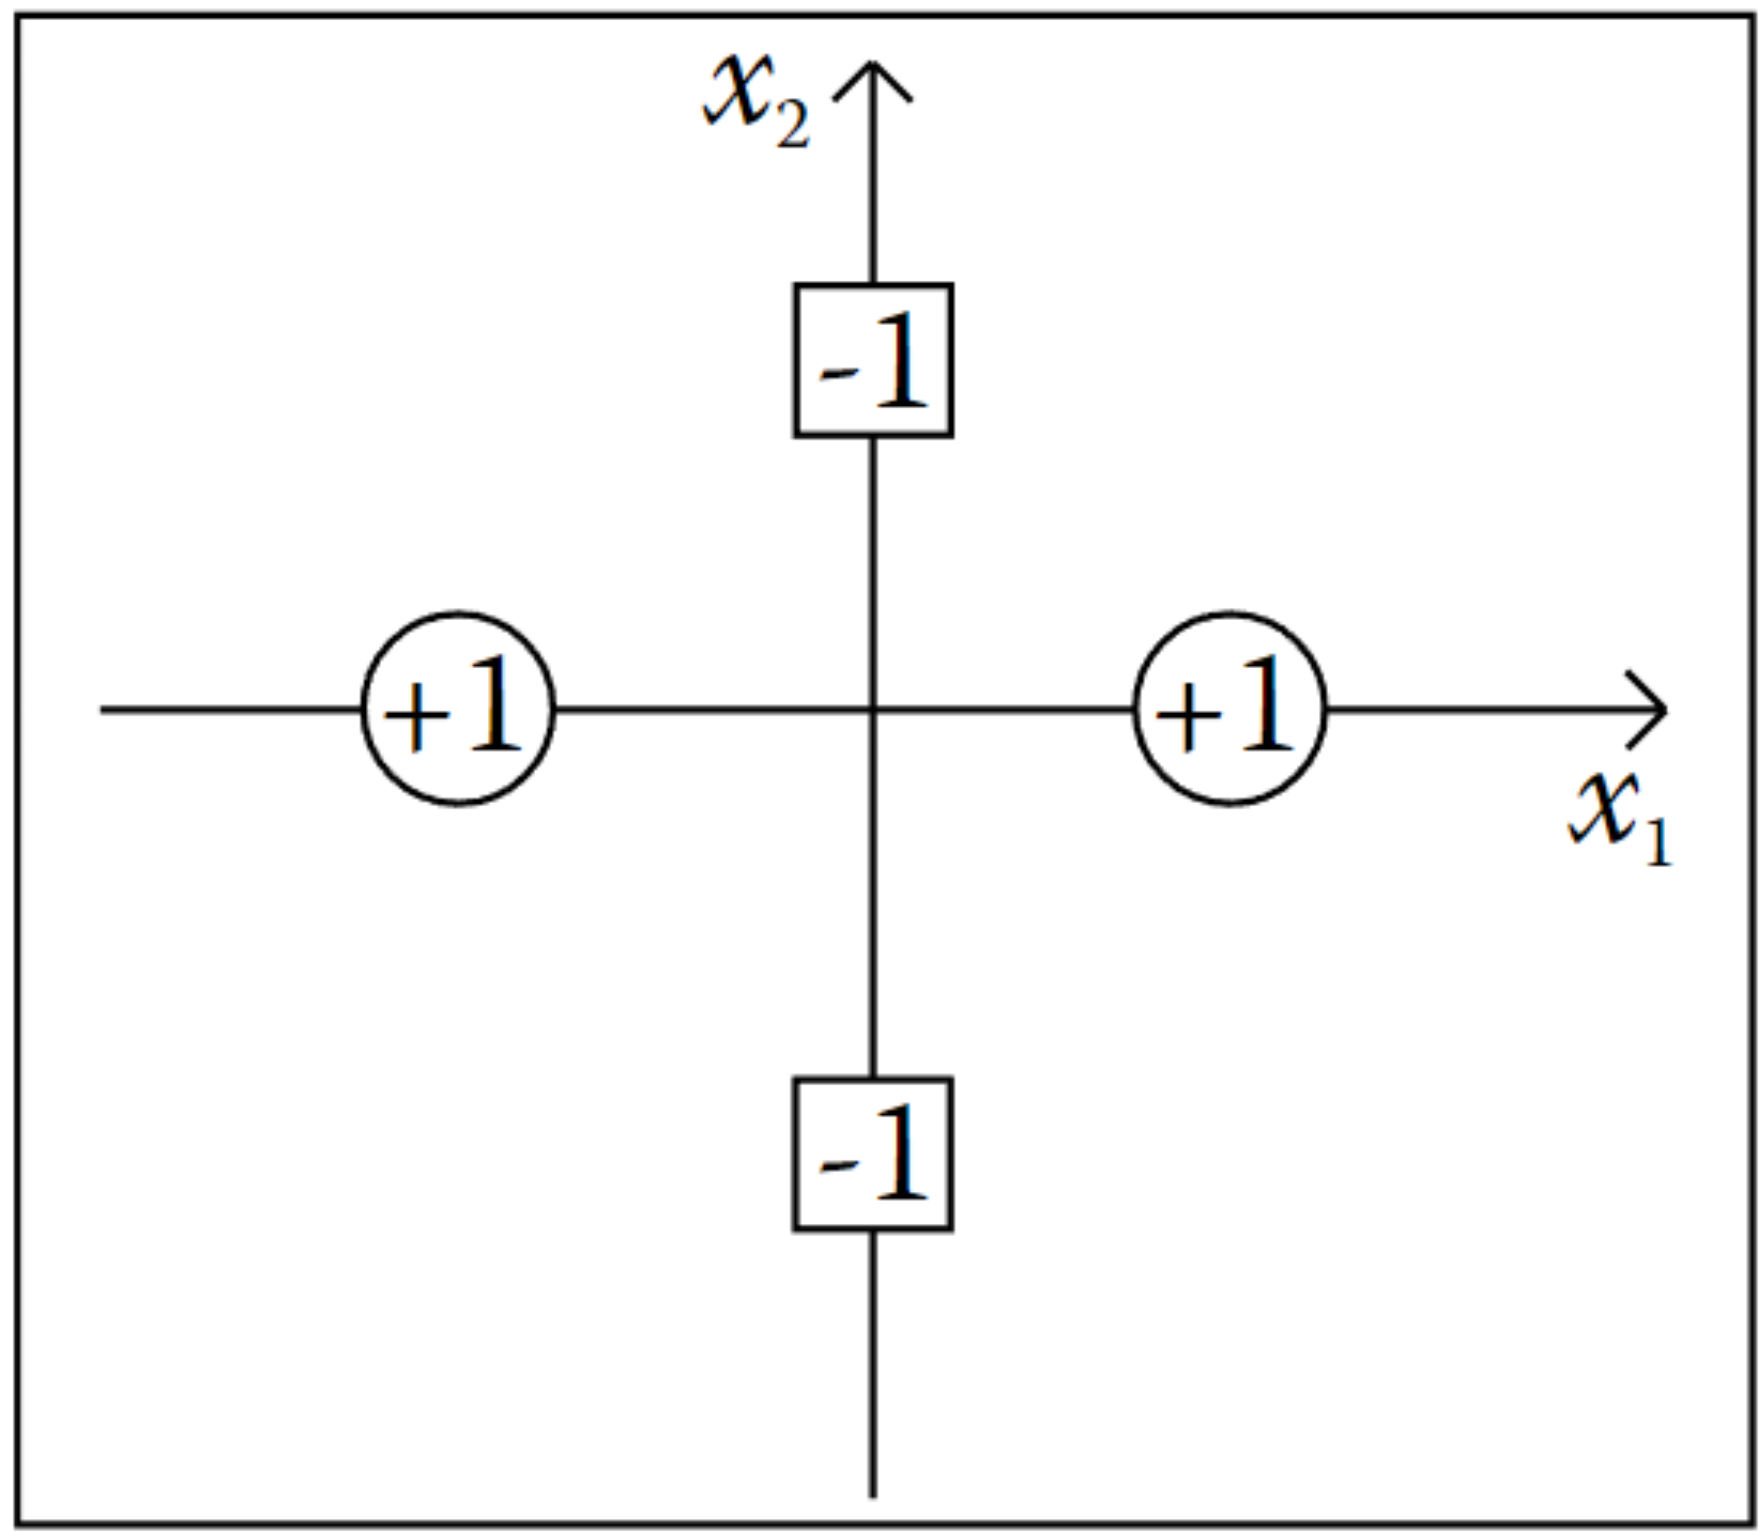
\includegraphics[width=0.5\textwidth]{../Ausarbeitung/figures/XOR-Problem.png}
\end{frame}

\section{Praktische Anwendung}
\begin{frame}{Praktische Anwendung und Beispiele}{\textbf{Bilderkennung und Computervision:} Gesichtserkennung}
	\begin{figure}
		\centering
		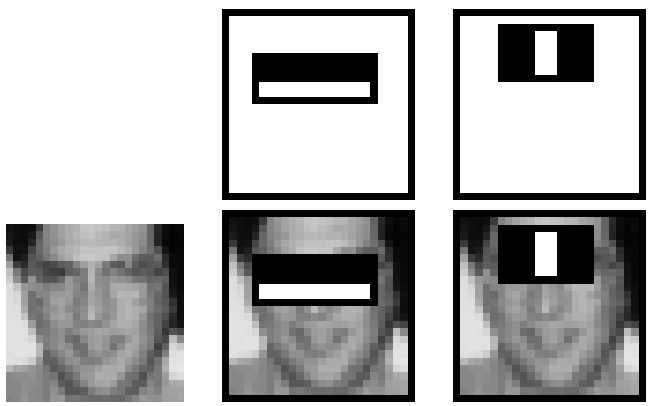
\includegraphics[width=0.7\textwidth]{../Ausarbeitung/figures/CV_Example.png}
	\end{figure}
\end{frame}
\begin{frame}{Praktische Anwendung und Beispiele}{\textbf{Textklassifikation und Natural Language Processing}: Erkennung von Spam-Mail}
	\begin{figure}
		\centering
		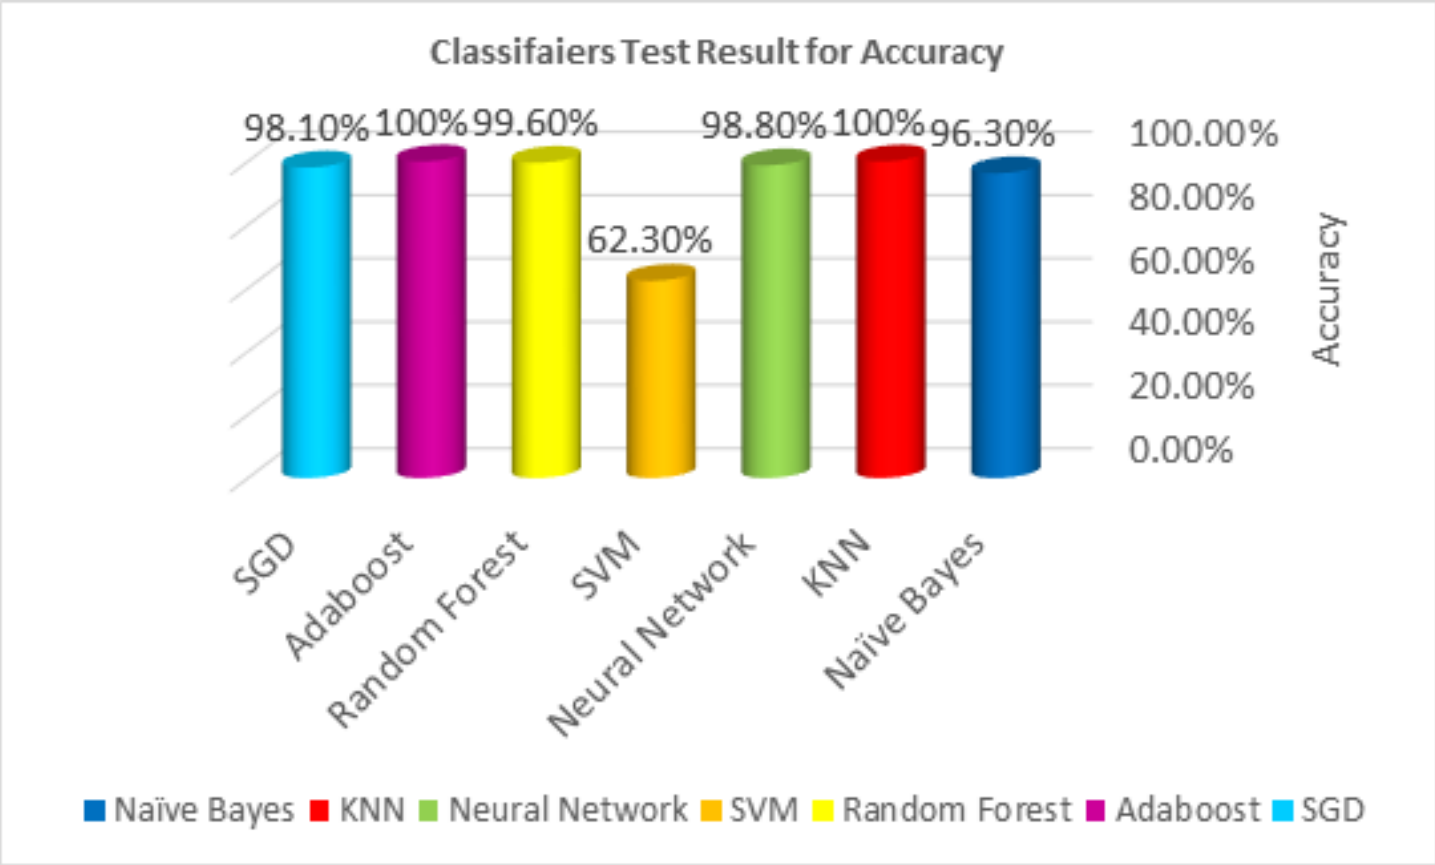
\includegraphics[width=0.7\textwidth]{../Ausarbeitung/figures/spam.png}
	\end{figure}
\end{frame}
\begin{frame}{Praktische Anwendung und Beispiele}{\textbf{Medizinische Diagnostik:} Risiko/Erkennung von Krankheiten baserend auf Patientendaten}
	\begin{figure}
		\centering
		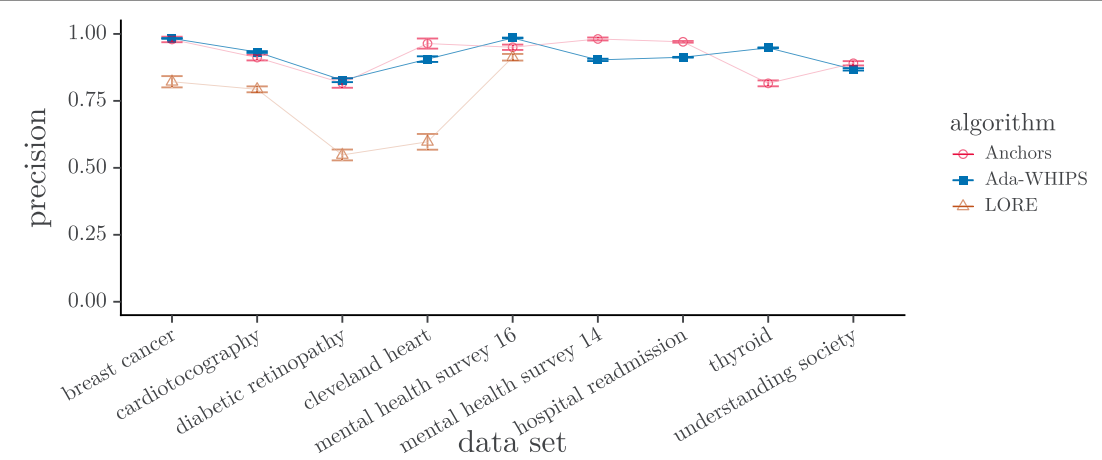
\includegraphics[width=\textwidth]{../Ausarbeitung/figures/ada-whips.png}
	\end{figure}
\end{frame}
\begin{frame}{Praktische Anwendung und Beispiele}{\textbf{Finanzwesen:} Vorhersage von Aktienkursbewegungen}
	\begin{figure}
		\centering
		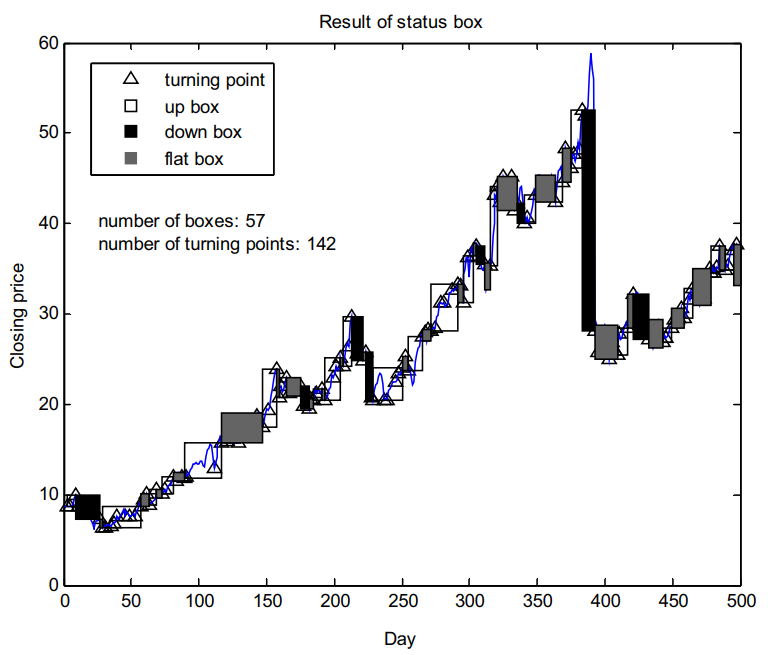
\includegraphics[width=0.7\textwidth]{../Ausarbeitung/figures/stock.png}
	\end{figure}
\end{frame}

\section{Vor- und Nachteile}
\begin{frame}{Vor- und Nachteile von AdaBoost}
	\begin{itemize}
		\item <1-> []\textbf{Vorteile:}\\[5pt]
		      \begin{itemize}
			      \item<2-> [\textbf{\textcolor{buwgreen}{+}}] Benutzerfreundlich
			      \item<3-> [\textbf{\textcolor{buwgreen}{+}}] Flexibel
			      \item<4-> [\textbf{\textcolor{buwgreen}{+}}] Identifiziert automatisch wichtige Features
			      \item<5-> [\textbf{\textcolor{buwgreen}{+}}] Neigt weniger zum Overfitting
		      \end{itemize}
		\item <6-> [] \textbf{Nachteile:}\\[5pt]
		      \begin{itemize}
			      \item<7-> [\textbf{\textcolor{darkred}{-}}] Anfällig für \textbf{verrauschte Daten und Ausreißer}
			      \item<8-> [\textbf{\textcolor{darkred}{-}}] Training auf großen Datensätzen kann \textbf{zeitintensiv} sein
			      \item<9-> [\textbf{\textcolor{darkred}{-}}] Hauptsächlich für \textbf{binäre Klassifikation} ausgelegt
		      \end{itemize}
	\end{itemize}
\end{frame}

\section{Erweiterungen und Variationen}
\begin{frame}{Erweiterungen und Variationen von AdaBoost}
	\begin{itemize}
		\item <1-> Ursprünglich für binäre Klassifikation entwickelt,
		      durch verschiedene Erweiterungen für diverse Problemstellungen adaptiert
		\item <2-> \glqq AdaBoost.M1\grqq~ und \glqq SAMME\grqq~ für \textbf{Multiklassen-Probleme}
		\item <3-> \textbf{Kosten-sensitives} AdaBoost
		\item <4-> Neben Decision Stumps kann AdaBoost mit \textbf{SVMs, Neuronalen Netzen und anderen Classifiern} kombiniert werden

	\end{itemize}
\end{frame}

\begin{frame}{Erweiterungen und Variationen von AdaBoost}
	\begin{itemize}
		\item <1-> \textbf{Robuste} Varianten minimieren die Auswirkung von Ausreißern.
		\item <2-> \textbf{Online} AdaBoost aktualisiert Modelle ohne Neutrainierung.
		\item <3-> \textbf{Direkte Feature Auswahl:} Wählt während des Trainings aus, welche Features wichtig sind
		      und betrachtet nur diese $\leadsto$ \textbf{schnelleres Training}
		\item <4-> Variationen, welche die \textbf{Interpretierbarkeit und Erklärbarkeit} verbessern
	\end{itemize}
\end{frame}
\section{Literatur und Zusatzmaterial}
\begin{frame}[allowframebreaks]{Literatur}
	\nocite{*}
	\bibliographystyle{alpha}
	\bibliography{../Ausarbeitung/seminar_top10.bib}
\end{frame}
\begin{frame}{Zusatzmaterial}
	\centering
	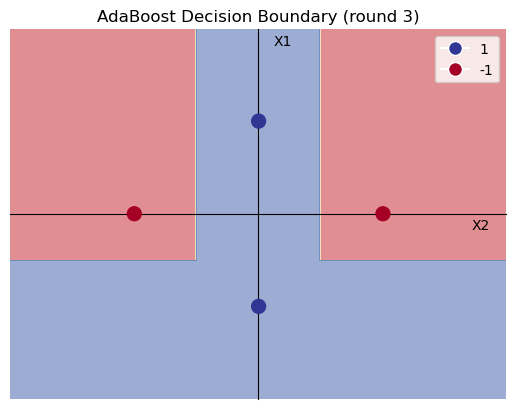
\includegraphics[width=0.45\textwidth]{../Code/img/XOR_Code.png}
	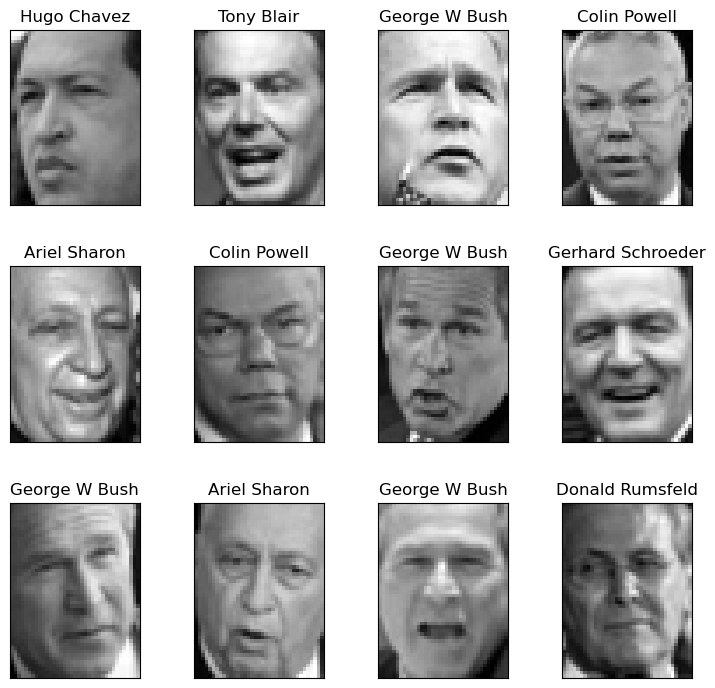
\includegraphics[width=0.45\textwidth]{../Code/img/face_recognition.png}\\
	Umsetzungen und Beispiele von AdaBoost + diese Präsentation mit Ausarbeitung
	in \LaTeX~auf \textcolor{buwgreen}{\emph{\underline{\href{https://github.com/Vinfeno/TTAIDM_AdaBoost}{GitHub}}}}.
\end{frame}

\begin{frame}{Danke}
	\resizebox{\linewidth}{!}{Vielen Dank für die Aufmerksamkeit!}
\end{frame}
\end{document}



